\section{Results and Evaluation}\label{sec:evaluation-results}

Table~\ref{tab:evaluation-scope} summarizes the scope of the reported evaluation and distinguishes measured outcomes from proposed extensions.
\begin{table}[htbp]
\centering\small
\caption{Evaluation scope and interpretation}
\label{tab:evaluation-scope}
\renewcommand{\arraystretch}{1.2}
\begin{tabularx}{\textwidth}{|Y|Y|Y|}
\hline
\textbf{Component} & \textbf{Reported evaluation} & \textbf{Interpretation} \\
\hline
Threat detector & Within-source held-out classification & Does not establish detection of unseen attacks or networks. \\
\hline
Threshold policy & Grid of 165 candidates; selected thresholds 0.30, 0.35, and 0.90 & Selection within the modeled policy space. \\
\hline
Allocator comparison & 30 held-out trace-derived scenarios & Profit, admission, and modeled exposure in a synthetic setting. \\
\hline
Admission control and algorithm selection & Objectives 2 and 3 remain proposed & No experimental performance claim is made for these objectives. \\
\hline
\end{tabularx}
\end{table}

\subsection{Threat Classification Accuracy}
The Random Forest classifier achieved strong results on a within-source held-out test set. As shown in the confusion matrix (Figure \ref{fig:confusion}), the model achieved near 100\% accuracy, precision, and recall. This within-source test does not establish robustness to new attacks or traffic distributions; false positives can still trigger costly isolation actions.

\begin{figure}[h!]
\centering
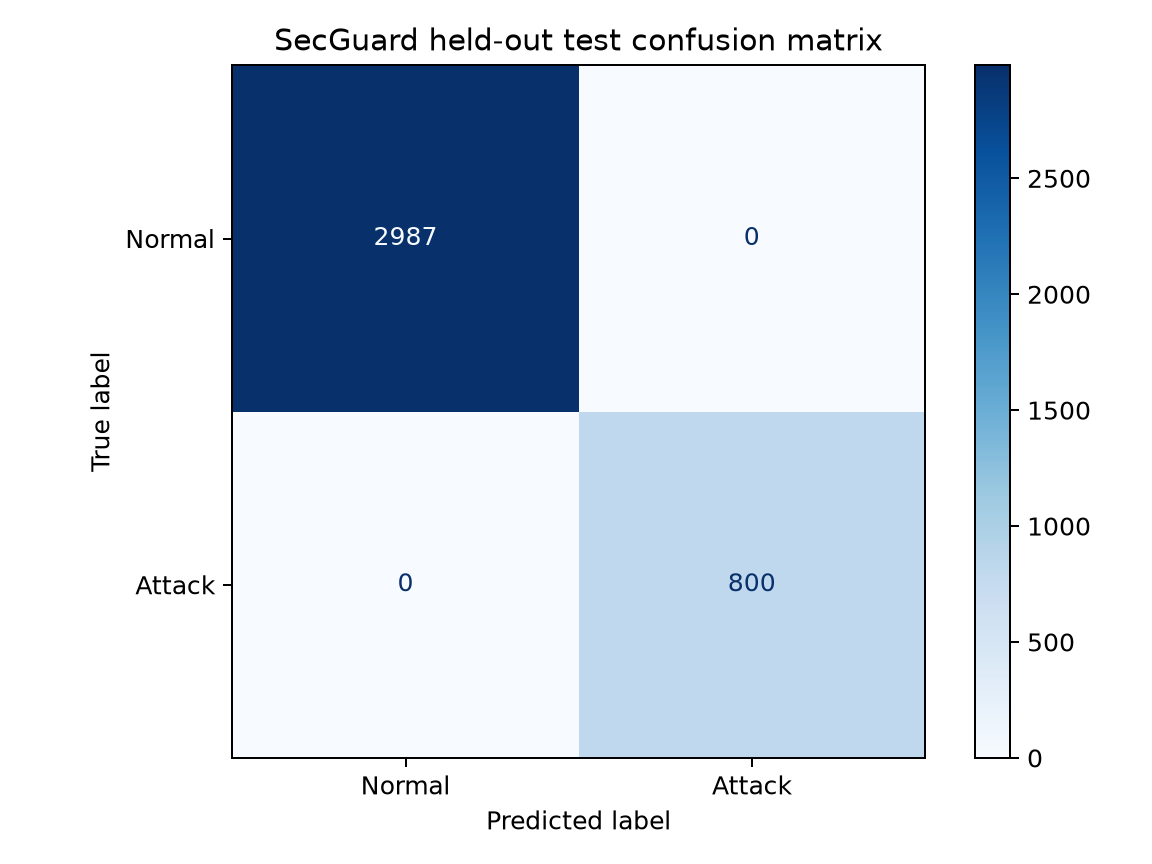
\includegraphics[width=0.6\textwidth]{confusion_matrix.png}
\caption{Confusion Matrix for Random Forest Packet Classifier}
\label{fig:confusion}
\end{figure}

\subsection{Surrogate Policy Pareto Frontier}
Figure \ref{fig:pareto} illustrates the threshold-policy trade-off over a grid of 165 candidates. The x-axis represents modeled isolation exposure (lower is better), and the y-axis represents InP profit (higher is better). The red curve shows the nondominated candidates in the plotted results.

From this frontier, the source report selected thresholds $\tau_{L1} = 0.30$, $\tau_{L2} = 0.35$, and $\tau_{quar} = 0.90$. The thresholds determine the simulated isolation action from the observed threat score.

\begin{figure}[h!]
\centering
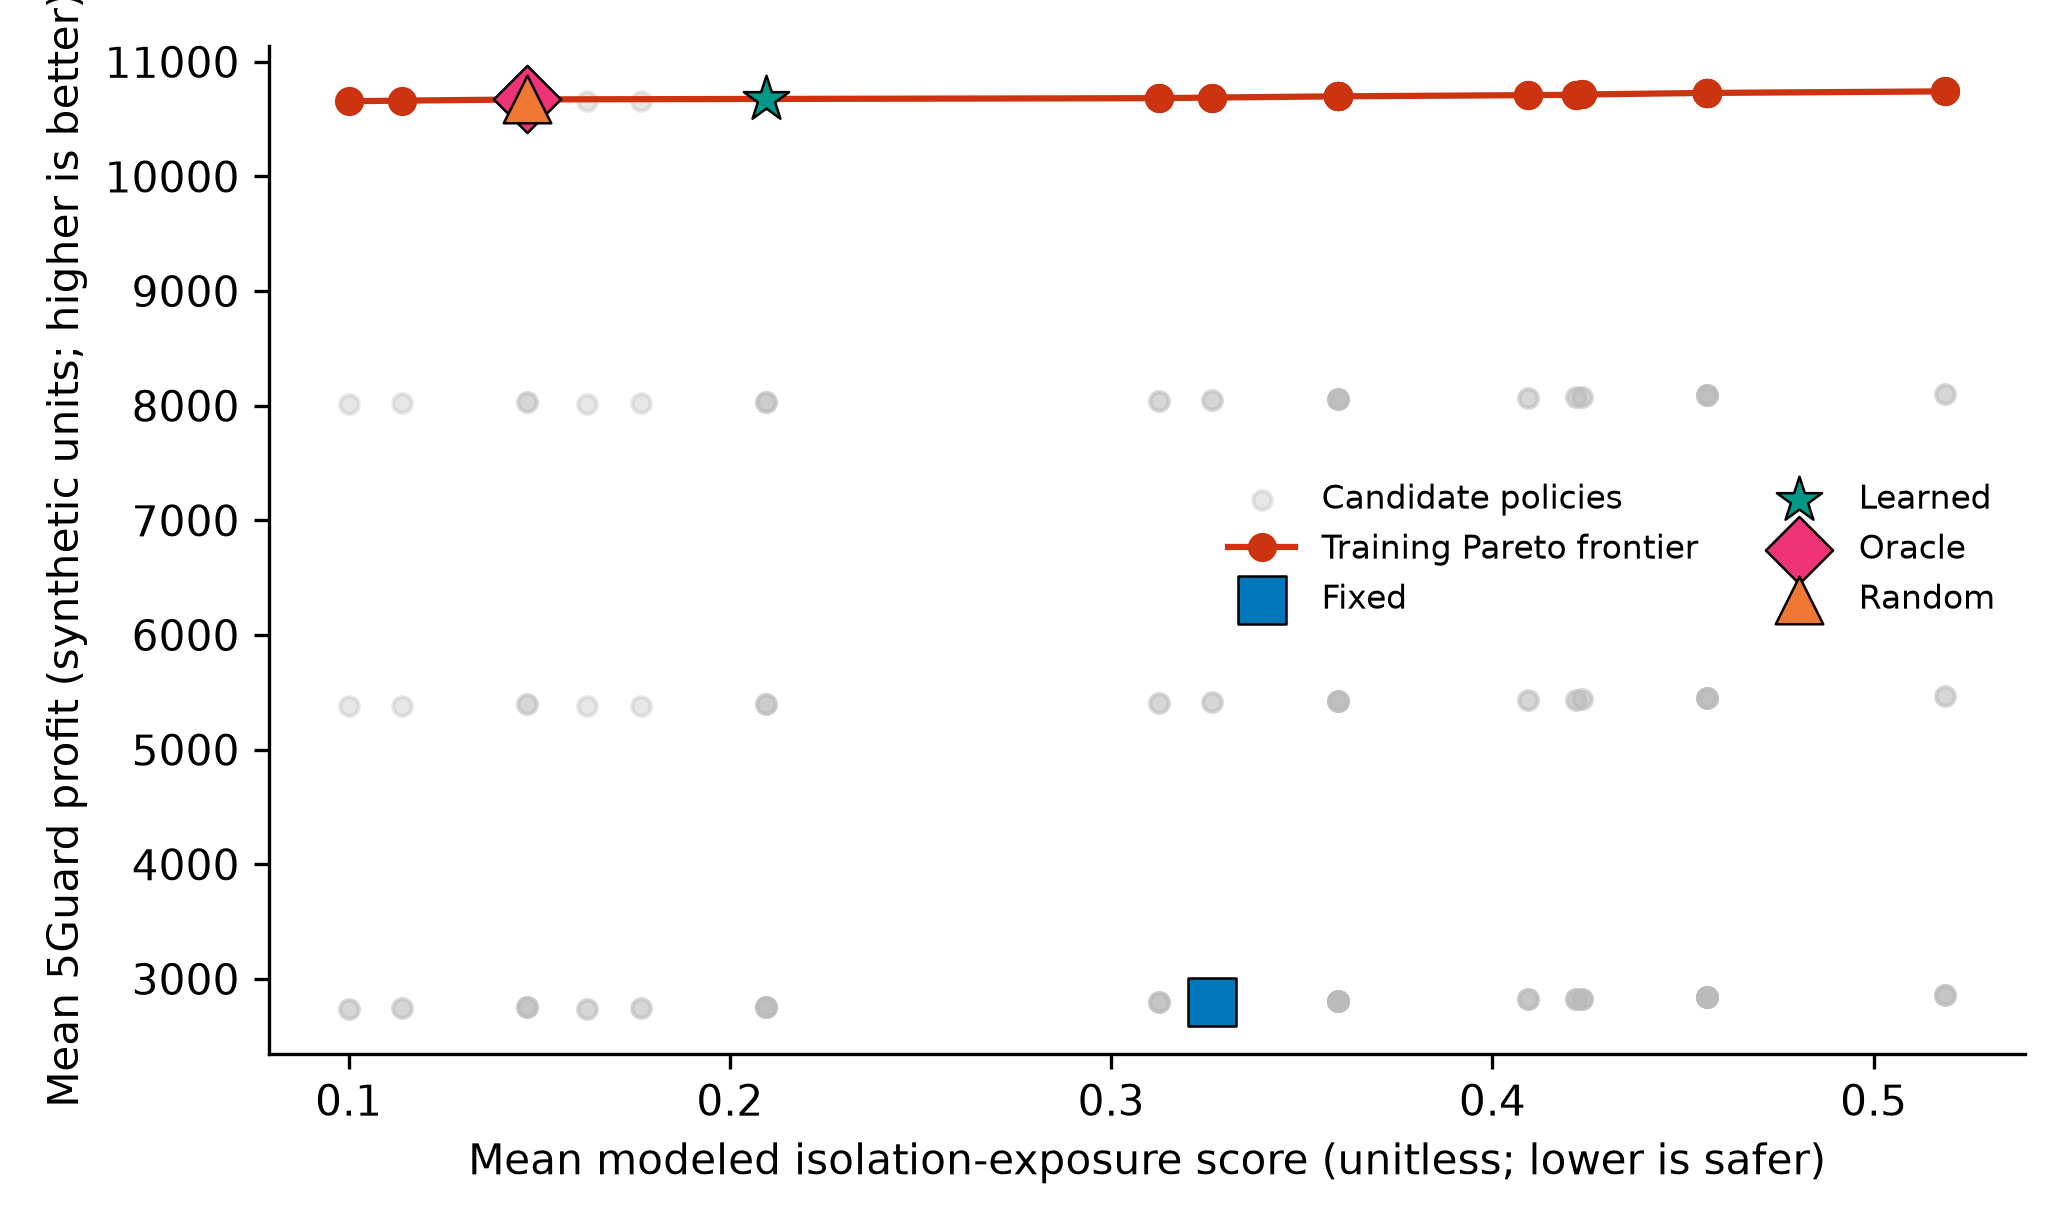
\includegraphics[width=0.7\textwidth]{pareto_frontier.png}
\caption{Pareto Frontier derived via Surrogate ML Optimization}
\label{fig:pareto}
\end{figure}

\subsection{End-to-End System Evaluation (Before vs. After)}
To rigorously validate Objective 1, we executed the 5Guard system across 30 held-out, trace-derived synthetic scenarios. We compared three distinct states:
\begin{enumerate}
    \item \textbf{Baseline 5Guard (No Security):} The original paper's logic. Isolation is purely based on static SLA requests.
    \item \textbf{Fixed SecGuard (Naive Rules):} A rigid security policy where thresholds are statically set without ML optimization.
    \item \textbf{Learned SecGuard (Our Work):} The system running our Pareto-optimal ML thresholds.
\end{enumerate}

\begin{table}[htbp]
\centering
\caption{Held-out policy results over 30 trace-derived scenarios}
\label{tab:policy-results}
\small
\begin{tabularx}{\textwidth}{Yrrrr}
\hline
\textbf{Policy} & \textbf{Mean profit} & \textbf{Exposure} & \textbf{Admitted} & \textbf{Quarantined} \\
\hline
Static 5Guard    & 8133.84 & 0.7729 & 3.00 & 0.00 \\
Fixed SecGuard   & 2776.79 & 0.2438 & 2.27 & 1.00 \\
Learned SecGuard & 7356.28 & 0.2542 & 2.90 & 0.30 \\
\hline
\end{tabularx}
\end{table}

\subsubsection{Statistical Improvements}
The preliminary comparison reports the following outcomes:
\begin{itemize}
    \item \textbf{Security Exposure Reduction:} Baseline 5Guard suffered a massive mean exposure score of 0.77. Our Learned SecGuard dropped this to 0.25, representing a \textbf{67.12\% reduction in the modeled isolation-exposure proxy}.
    \item \textbf{Profit Recovery:} The Fixed SecGuard (naive rules) over-reacted to threats, resulting in massive L2 over-provisioning and quarantines, plunging the mean profit to 2,776.7. Our Learned SecGuard intelligently balanced the risk, achieving a mean profit of 7,356.2, representing a \textbf{164.9\% higher mean profit relative to the fixed policy}.
    \item \textbf{Profit Retention:} The selected policy retained \textbf{90.4\%} of the static baseline mean profit in this evaluation.
    \item \textbf{Admission Rate:} The Learned policy admitted an average of 2.9 out of 4 slices per scenario, compared to only 2.2 for the naive policy, indicating higher admission in these scenarios.
\end{itemize}

\begin{figure}[h!]
\centering
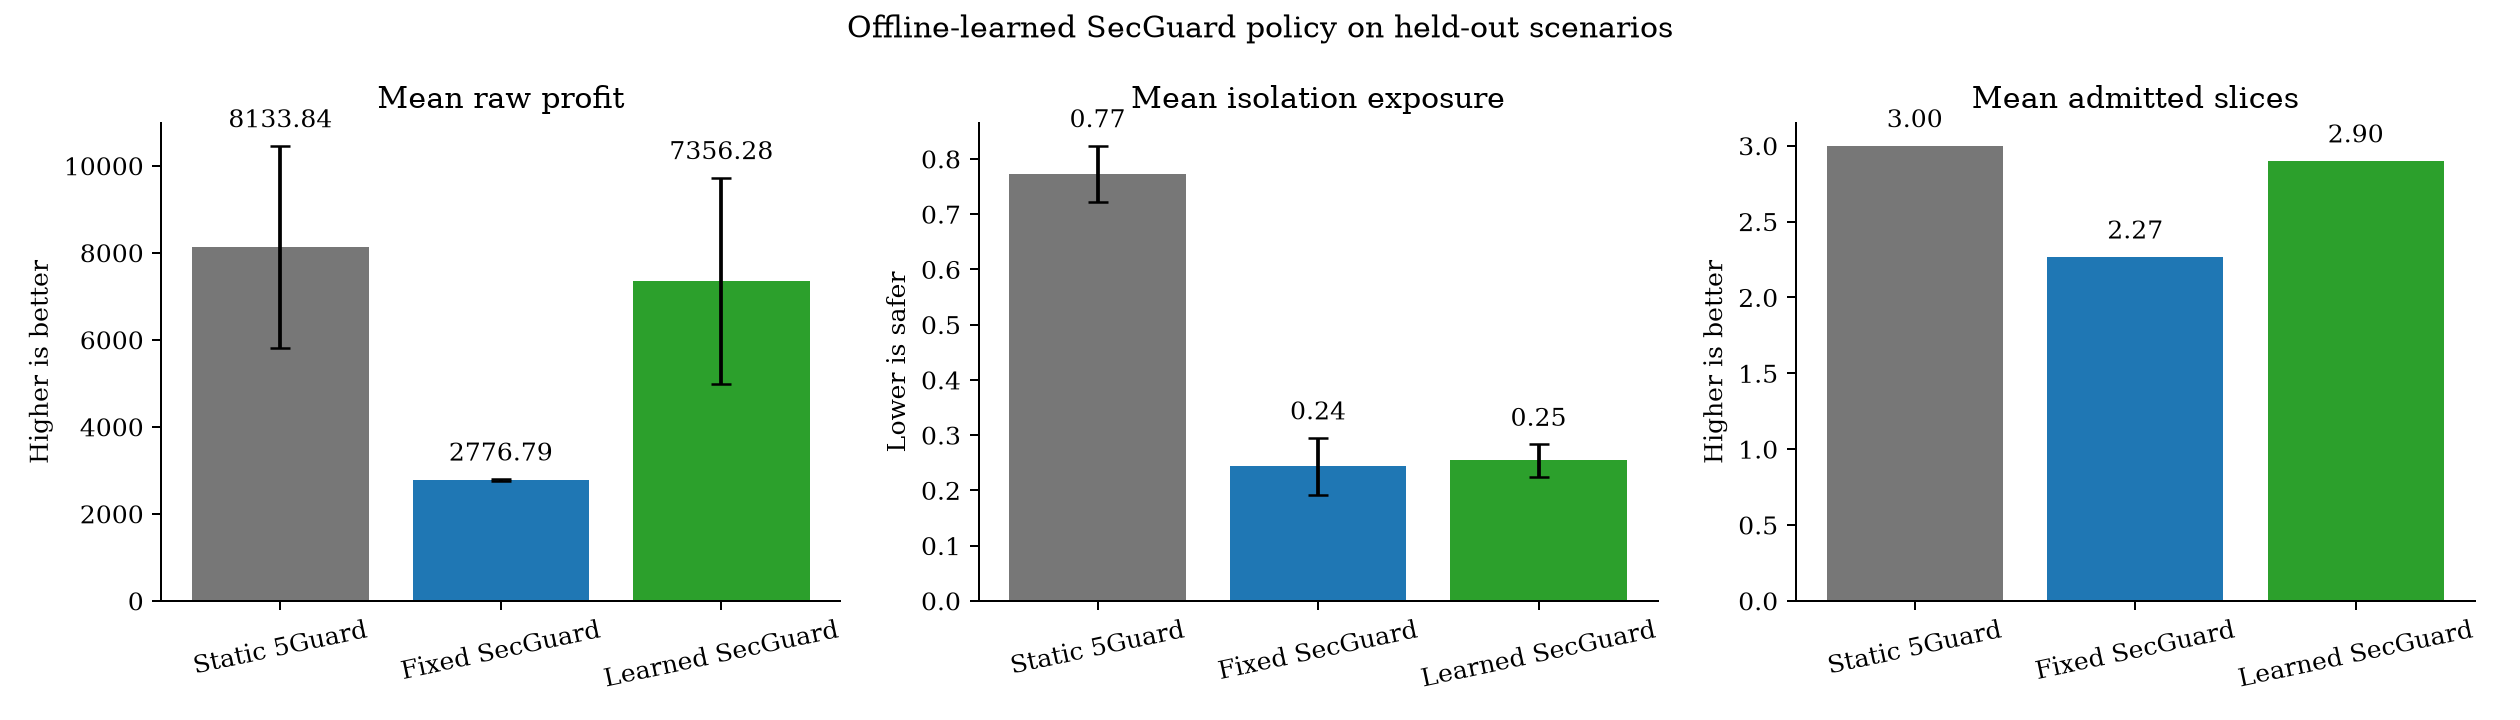
\includegraphics[width=0.7\textwidth]{learned_policy_comparison.png}
\caption{Comparison of Profit vs Security Exposure across Policies}
\label{fig:comparison}
\end{figure}

\subsection{The Security-Resource Efficiency (SRE) Metric}
For future evaluation, the source report proposes a \textbf{Security-Resource Efficiency (SRE)} measure. 
\begin{equation}
    SRE = \frac{\Delta \text{Exposure Reduction}}{\Delta \text{Isolation Overhead}}
\end{equation}
SRE requires a consistent isolation-overhead definition and should be evaluated separately before drawing an optimization claim.

\clearpage
\section{Limitations and Future Work}\label{sec:limitations}

While Objective 1 of SecGuard shows promising preliminary results, several limitations must be acknowledged:

\subsection{Adversarial Machine Learning}
The Random Forest classifier relies on standard telemetry features. Advanced attackers could utilize Adversarial ML techniques to artificially alter packet flow timings and payload sizes, effectively hiding malicious traffic below the classifier's decision boundary. Future work must incorporate robust, adversarial-aware training protocols.

\subsection{Generalization to Complex Topologies}
The MILP and heuristic simulations were executed on a medium-scale topology consisting of interconnected Edge and Core nodes. Scaling the exact MILP solver to nation-wide topologies (thousands of nodes) remains computationally intractable. This highlights the urgent necessity of \textbf{Objective 3 (Intelligent Algorithm Selection)} to intelligently route requests away from the exact solver when the graph size crosses critical complexity thresholds.

\subsection{Reinforcement Learning Stability (Objective 2)}
The proposed Deep Q-Network for Admission Control (Objective 2) faces significant challenges regarding training stability. The 5G network state space is highly stochastic and non-stationary. Future iterations of this work will explore Proximal Policy Optimization (PPO) and Multi-Agent RL to stabilize convergence.

\section{Conclusions}\label{sec:conclusions}
The preliminary evaluation reports a 67.12\% reduction in the modeled isolation-exposure proxy while retaining 90.4\% of the static baseline mean profit. These results support further investigation of risk-adaptive isolation. They do not yet establish attack containment or performance on a deployed network.

Objectives 2 and 3 remain future work. They require dedicated training and held-out evaluation before claims about admission quality or allocation latency can be made.
